%%%%%%%%%%%%%%%%%%%%%%%%%%%%%%%%%%%%%%%%%
%
% Funkcionalna verifikacija hardvera
% 
%%%%%%%%%%%%%%%%%%%%%%%%%%%%%%%%%%%%%%%%%

Deveta vežba je posvećena hijerarhiji UVM verifikacionog okruženja. Dat je
pregled UVM agent klase, često korišćene klase za konfiguraciju kao i UVM
environment klase. Objašnjen je \emph{factory override} mehanizam i dat primer
upotrebe.

%========================================================================================
% Section
%========================================================================================

\section{Agent}

Iako se drajver, sekvencer i monitor mogu koristiti nezavisno to iziskuje
poznavanje imena, uloge i načina povezivanja svake komponente. Agent obuhvata
ove tri komponente, predstavlja apstraktniji pristup datom interfejsu i olakšava
ponovno korišćenje ovih komponenti. Može biti aktivni ili pasivni. Aktivni
agenti sadrže komponente koje generišu stimulus na interfejsu kao i one koje ga
nadgledaju, dok pasivni agenti samo nadgledaju interfejs odnosno pasivni agenti
sadrže samo monitor zbog čega je veoma bitno da su drajver i monitor potpuno
odvojeni iako im je deo funkcionalnosti sličan. Pasivni agenti se uglavnom
koriste kao mali deo nekog većeg okruženja kada se stimulus generiše iz neke
druge komponente.

\begin{figure}[h!]
  \centering
  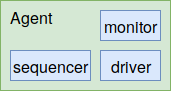
\includegraphics[width=40mm, scale=0.5]{img/v9_agent.png}
  \caption{Agent}
  \label{fig:agent}
\end{figure}

% ----------------------------------------------------------------------------------------

\subsection{Struktura}

Kao što je već rečeno agent vrši povezivanje monitora, sekvencera i drajvera
koristeći TLM konekcije. Kako bi se olakšala upotreba i fleksibilnost agenta, on
sadrži i konfiguracione informacije smeštene u posebnom objektu.\\

Agent ima dva režima rada:

\begin{itemize}
\item Aktivni režim - agent generiše DUT signale; u ovom režimu agent instancira
  drajver i sekvencer, kao i monitor
\item Pasivni režim - agent samo nadgleda signale; u ovom režimu agent ne
  instancira drajver i sekvencer, već samo monitor
\end{itemize}

U nastavku je dat primer agenta. Implementacija se vrši nasleđivanjem
\emph{uvm\(\_\)agent} klase, sadrži kod za \emph{factory} registraciju i
konstruktor koji prate klasični UVM mehanizam.

\lstinputlisting[caption=Kostur agenta, label=lst:calc_agent]{code/v9_calc_agent.sv}

Agent u \emph{build} fazi uvek kreira monitor, a kreira drajver i sekvencer
jedino ukoliko je odabran aktivni režim rada. Sve komponente se kreiraju
koristeći preporučeni metod, a ne direktno pozivanjem konstruktora \emph{new}.
Takođe će se drajver i sekvencer u \emph{connect} fazi povezati jedino u
aktivnom režimu rada.

% ----------------------------------------------------------------------------------------

\subsection{Konfiguracija}

Odabir režima rada, kao i sve opcije vezane za konfiguraciju agenta, obično se
nalaze u posebnom objektu koji se prosleđuje koristeći
\emph{uvm\(\_\)config\(\_\)db}. Preuzimanje iz baze se vrši u \emph{build} fazi:

\begin{lstlisting}
if(!uvm_config_db#(calc_config)::get(this, "", "calc_config", cfg))
      `uvm_fatal("NO_CFG",{"Config object must be set for: ",get_full_name(),".cfg"})
\end{lstlisting}

Sama konfiguraciona klasa se implementira nasleđivanjem \emph{uvm\(\_\)object}
klase, sadrži \emph{factory} registraciju i konstruktor pisani po već
objašnjenim pravilima i može sadržati proizvoljna polja u zavisnosti od potreba
datog agenta. U nastavku je dat primer:

\lstinputlisting[caption=Primer konfiguracije agenta, label=lst:calc_config]{code/v9_calc_config.sv}

Polje koje se skoro uvek sreće u konfiguraciji agenta je za odabir režima rada.
Zbog ovoga postoji predefinisani nabrojivi tip
\emph{uvm\(\_\)active\(\_\)passive\(\_\)enum} i konvencija je da se koristi za
ovu funkcionalnost. Može imati vrednosti UVM\(\_\)ACTIVE ili UVM\(\_\)PASSIVE.

\begin{lstlisting}
// Enum: uvm_active_passive_enum
//
// Convenience value to define whether a component, usually an agent,
// is in "active" mode or "passive" mode.
typedef enum bit { UVM_PASSIVE=0, UVM_ACTIVE=1 } uvm_active_passive_enum;
\end{lstlisting}

Pored ovog polja ova klasa može sadržati bilo koja polja potrebna za podešavanje
konfiguracije agenta - npr. da li da se sakupljaju podaci o pokrivenosti ili ne,
da li da se vrši čekiranje ili ne, \emph{baud rate}, odabir \emph{parity}
režima, CRC režima i sl.\\

Konfiguracioni objekat se kreira i podešava na višem nivou hijerarhije (npr. u
testu), a zatim se preko baze prosleđuje agentu. Npr:

\begin{lstlisting}
calc_config cfg;
// ...
function void build_phase(uvm_phase phase);
  // ...
  cfg = calc_config::type_id::create("cfg");
  uvm_config_db#(calc_config)::set(this, "*", "calc_config", cfg);
endfunction : build_phas
\end{lstlisting}

%========================================================================================
% Section
%========================================================================================

\section{Hijerarhija okruženja}

UVM verifikaciona okruženja se grade iz klasa koje nasleđuju
\emph{uvm\(\_\)component} klasu. Hijerarhija je određena nizom \emph{has-a}
klasnih veza gde jedna komponeta instancira druge, podkomponente. Na najvišem
nivou se nalazi sam test u kome se vrši odabir konfiguracije okruženja,
kreiranje svih podkomponenti, startovanje sekvenci, ... Sama arhitektura
okruženja je uglavnom konstantna i modularna kako bi se omogućila laka ponovna
upotreba verifikacionih komponenti (bilo horizontalna, bilo vertikalna). U UVM-u
postoje dve komponente koje služe za grupisanje i olakšavanje ponovne upotrebe.
Njihova uloga je jedino organizacija okruženja i definisanje jasne hijerarhije.
Ove dve klase su agenti tj. \emph{uvm\(\_\)agent} (opisani u prethodnom
poglavlju) i okruženja tj. \emph{uvm\(\_\)env}.

% ----------------------------------------------------------------------------------------

\subsection{Blok nivo}

Ovaj nivo zapravo predstavlja \emph{environment} klasu koja grupiše sve
komponente za ponovnu upotrebu. U njoj se vrši konfiguracija svih podkomponenti.
Većina ponovne upotrebe se vrši na ovom nivou odnosno korisnik instancira datu
\emph{uvm\(\_\)env} klasu i konfiguriše agente prema svojim potrebama.
\emph{Env} klasa obično sadrži konfiguracionu klasu i željeni broj agenata,
prikazano na slici \ref{fig:block_env}.\\

\begin{figure}[h!]
  \centering
  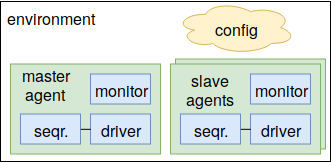
\includegraphics[width=80mm]{img/v9_block_env.png}
  \caption{UVM env}
  \label{fig:block_env}
\end{figure}

Umesto pojedinačnog instanciranja svih podkomponenti i podešavanja režima rada
svake od njih, korišćenjem komponenti za grupisanje (agent i \emph{env})
omogućava se podizanje nivoa hijerarhije i olakšava upotreba, ukoliko su sve
komponente kreirane prateći UVM metodologiju. Upotreba od strane korisnika mora
biti jasno definisana tj. opcije konfiguracije treba da su dobro
dokumentovane.\\

Klasičan primer upotrebe bile bi komponente za protokole npr. AXI, UART, SPI,
... Prilikom verifikacije dizajna koji implementira neki protokol, korisnik bi
instancirao datu klasu i promoću konfiguracije kontrolisao strukturu - da li je
potreban master ili \emph{slave} agent, broj agenata, da li su aktivni ili
pasivni itd. Ovim se eleminiše potreba za detaljnim poznavanjem implementacije
samih komponenti i omogućava brz i jednostavan način kreiranja kompleksnih
okruženja. Ovakve komponente se obično nazivaju protokol UVC (UVM Verification
Component) i najčešći su primer ponovne upotrebe koda u verifikacionim
okruženjima.

% ----------------------------------------------------------------------------------------

\subsection{\emph{Top-level} okruženje}

Kao što je već rečeno na najvišem nivou hijerarhije se nalazi test klasa.
Međutim, radi preglednosti i jasne organizacije koda, obično postoji i jedno
okruženje koje obuhvata sve podkomponente i koje se instancira u samom testu.
Tada se test fokusira samo na kreiranje sekvenci i podešavanje konfiguracija, a
sva instanciranja i povezivanja podkomponenti se vrše u \emph{env} klasi. Ovo
\emph{top-level} okruženje se često naziva i testbenč.\\

\emph{Top-level} okruženje uglavnom sadrži određeni broj agenata (direktno ili
preko okruženja opisanih u prethodnom poglavlju), ali sadrži i sve ostale
komponente potrebne za proveru rada DUT-a npr. \emph{scoreboard}-e, globalne
monitore, prikupljače pokrivenosti, ... Obično sadrži i konfiguracionu klasu
preko koje se mogu podešavati određene osobine npr. konfiguracije samih
agenata.\\

Na slici \ref{fig:top_env} je prikazan blok dijagram klasičnog UVM
verifikacionog okruženja. \emph{Env} klasa sadrži SPI i APB agent,
\emph{scoreboard} povezan sa oba monitora preko TLM interfejsa, i monitor za
prikupljanje pokrivenosti povezan sa APB monitorom. \emph{Env} takođe sadrži i
konfiguracionu klasu preko koje je moguće pristupati konfiguracijama APB i SPI
agenata. U testu je jedino potrebno instancirati \emph{env} klasu, eventualno
podesiti konfiguraciju i zatim pokretati sekvence na APB i SPI sekvencerima.

\begin{figure}[h!]
  \centering
  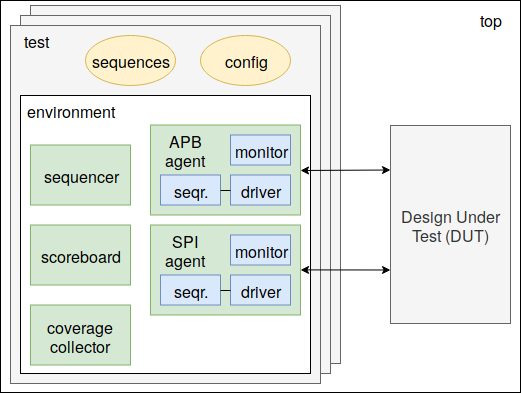
\includegraphics[width=100mm]{img/v9_top_env.png}
  \caption{Primer okruženja}
  \label{fig:top_env}
\end{figure}

%========================================================================================
% Section
%========================================================================================

\section{\emph{Factory override}}

UVM \emph{factory} omogućava da se jedna klasa zameni drugom, izvedenom klasnom
kada se konstruiše. Ovaj mehanizam može biti veoma korisan za promenu ponašanja
testbenča bez potrebe da se modifikuje ili rekompajlira kod. Kako bi ovo bilo
moguće potrebno je pratiti sve konvencije kodovanja opisane u petoj vežbi.\\

UVM \emph{factory} se može posmatrati kao \emph{lookup} tabela. Kada se
komponente konstruišu koristeći \emph{\textless type\textgreater
  ::type\(\_\)id::create("\textless name\textgreater ", \textless
  parent\textgreater )} pristup, tada se \emph{type\(\_\)id} koristi kako bi se
odabrao \emph{wrapper} za klasu, izvršila konstrukcija i vratio pokazivač.
Korišćenjem \emph{override} mehanizma se originalni \emph{type\(\_\)id}
zamenjuje drugim i time se vraća pokazivač na drugi objekat. Čitava tehnika je
zasnovana na polimorfizmu tj. mogućnosti da se izvedeni tipovi referenciraju
koristeći bazni pokazivač. Ovo znači da \emph{override} može da se koristi
jedino da se \emph{parent} klasa zameni sa nekom njenom \emph{child} klasom.\\

U UVM-u se \emph{override} može koristiti i za komponente i za objekte, što je
opisano u nastavku.

Komponente se mogu zameniti na dva načina - preko tipa ili preko instance.
Zamena preko tipa znači da će se prilikom svakog kreiranja date komponente
zapravo koristiti druga klasa, odnosno zamena se odnosi na sve instance date
komponente u okruženju. Takođe je moguće zameniti samo jednu instancu, a ne
sve. Ovo je često korisno prilikom korišćenja parametrizovanih klasa kako bi se
jednostavno promenila vrednost parametra.\\

Postoje dve UVM funkcije koje služe za \emph{override}:

\begin{lstlisting}
<original_type>::type_id::set_type_override(<substitute_type>::get_type(), bit replace = 1);
<original_type>::type_id::set_inst_override(<substitute_type>::get_type(),string <path_string>);
\end{lstlisting}

Gde je \emph{\textless original\(\_\)type\textgreater} tip komponente koju
želimo da zamenimo sa \emph{\textless substitute\(\_\)type\textgreater}, a
\emph{replace} je bit koji dozvoljava zamenu već postojeće zamene ukoliko ima
vrednost 1, a koristi se već postojeća zamena ukoliko ima vrednost 0.
\emph{\textless path\(\_\)string\textgreater} prilikom zamene instance
predstavlja putanju do instance koju treba zameniti.\\

U nastavku je dat jednostavan primer:

\begin{lstlisting}
class colour extends uvm_component;
  `uvm_component_utils(colour)
  // etc
endclass: colour

class red extends colour;
  `uvm_component_utils(red)
  //etc
endclass: red

// zamena svih instanci tipa "colour" sa "red":
colour::type_id::set_type_override(red::get_type(), 1);

// odnosno svaki poziv naredne linije vraca "red", a ne "colour"
pixel = colour::type_id::create("pixel", this);

// druga mogucnost - zamena samo jedne instance
// koja se nalazi na putanji "uvm_test_top.env.spot"
colour::type_id::set_inst_override(red::get_type(), "uvm_test_top.env.spot");
\end{lstlisting}

Za zamenu objekata se generalno koristi jedino zamena tipa, pošto za objekte ne
postoji hijerarhija kao za komponente na kojoj se zasniva mehanizam zamene
instanci. Kod je isti kao i za komponente.

%========================================================================================
% Section
%========================================================================================

\section{Zadaci}

\paragraph{Zadatak}

U pratećim materijalima za vežbu je dat kostur okruženja za ``Calc1'' dizajn.
Korišćene su \emph{uvm\(\_\)agent} i \emph{uvm\(\_\)env} klase. Proučiti
strukturu okruženja. Gde su i kako kreirane podkomponente? Šta može sadržati
\emph{calc\(\_\)config} klasa?

\paragraph{Zadatak}

U pratećim materijalima za vežbu je dat fajl
``factory\(\_\)override\(\_\).sv'' u kome se nalazi primer korišćenja
mehanizma zamene za objekte i komponente. Analizirati dati kod. Koji tipovi će
se koristiti u \emph{env} klasi? Modifikovati test tako da se jedino za a2
komponentu u \emph{env}-u koristi \emph{A\(\_\)ovr} tip, dok za sve ostale
komponente (\emph{a1} u ovom slučaju) koristi \emph{A} klasa.

\paragraph{Zadatak}

Za razvijeno okruženje za ``Calc1'' implementirati novu klasu za
\emph{sequence\(\_\)item}, koja nasleđuje već razvijenu klasu. Nova transakcija
treba da sadrži ograničenje da se nikad ne koristi operacija oduzimanja.
Napisati test koji će u čitavom okruženju koristiti novu klasu.

%========================================================================================
% Section
%========================================================================================

\section{Appendix}

\lstinputlisting[caption=v9\(\_\)factory\(\_\)override, label=lst:v9_factory_override]{code/v9_factory_override.sv}
\lstinputlisting[caption=calc\(\_\)if, label=lst:calc_if]{code/calc_if.sv}

\lstinputlisting[caption=v9\(\_\)calc\(\_\)agent, label=lst:v9_agent]{code/v9_calc_agent.sv}
\lstinputlisting[caption=v9\(\_\)calc\(\_\)config, label=lst:v9_config]{code/v9_calc_config.sv}
\lstinputlisting[caption=v9\(\_\)calc\(\_\)driver, label=lst:v9_driver]{code/v9_calc_driver.sv}
\lstinputlisting[caption=v9\(\_\)calc\(\_\)env, label=lst:v9_env]{code/v9_calc_env.sv}
\lstinputlisting[caption=v9\(\_\)calc\(\_\)seq\(\_\)item, label=lst:v9_seq_item]{code/v9_calc_seq_item.sv}
\lstinputlisting[caption=v9\(\_\)calc\(\_\)monitor, label=lst:v9_monitor]{code/v9_calc_monitor.sv}
\lstinputlisting[caption=v9\(\_\)calc\(\_\)sequencer, label=lst:v9_sequencer]{code/v9_calc_sequencer.sv}
\lstinputlisting[caption=v9\(\_\)test\(\_\)base, label=lst:v9_test_base]{code/tests/v9_test_base.sv}
\lstinputlisting[caption=v9\(\_\)test\(\_\)simple, label=lst:v9_test_simple]{code/tests/v9_test_simple.sv}
\lstinputlisting[caption=v9\(\_\)test\(\_\)simple\(\_\)2, label=lst:v9_test_simple_2]{code/tests/v9_test_simple_2.sv}
\lstinputlisting[caption=v9\(\_\)test\(\_\)lib, label=lst:v9_test_lib]{code/tests/v9_test_lib.sv}
\lstinputlisting[caption=v9\(\_\)calc\(\_\)base\(\_\)seq, label=lst:v9_calc_base_seq]{code/sequences/v9_calc_base_seq.sv}
\lstinputlisting[caption=v9\(\_\)calc\(\_\)simple\(\_\)seq, label=lst:v9_calc_simple_seq]{code/sequences/v9_calc_simple_seq.sv}
\lstinputlisting[caption=v9\(\_\)calc\(\_\)seq\(\_\)lib, label=lst:v9_calc_seq_lib]{code/sequences/v9_calc_seq_lib.sv}
\lstinputlisting[caption=v9\(\_\)calc\(\_\)verif\(\_\)pkg, label=lst:v9_calc_verif_pkg]{code/v9_calc_verif_pkg.sv}
\lstinputlisting[caption=v9\(\_\)calc\(\_\)verif\(\_\)top, label=lst:v9_calc_verif_top]{code/v9_calc_verif_top.sv}
\lstinputlisting[language=tcl, caption=calc\(\_\)run, label=lst:calc_run]{code/calc_run.do}